%Set document class
\documentclass{article}

%Load math symbol packages
\usepackage{amsmath}
\usepackage{amssymb}
\usepackage{mathtools}
\usepackage{indentfirst}
\usepackage{graphicx}
\usepackage{listings}

%User defined commands
\newcommand{\var}{\operatorname{Var}}
\newcommand{\cov}{\operatorname{Cov}}
\newcommand{\sumN}{\sum_{i=1}^{n}}
\newcommand{\sumM}{\sum_{i=1}^{m}}
\newcommand{\prodN}{\prod_{i=1}^{n}}
\newcommand{\prodM}{\prod_{i=1}^{m}}

\begin{document}
\begin{center}
	\huge{\bf Math 181B: Homework 2} \\
	Merrick Qiu 
\end{center}

\subsection*{Exercise 1}
\begin{enumerate}
	\item \begin{lstlisting}
getf = function() {
	sampleX = rnorm(50, mean=1, sd=2)
	sampleY = rnorm(50, mean=0, sd=2)
	varX = var(sampleX)
	varY = var(sampleY)
	f = varY/varX
	return(f)
}

fvalues = rep(0, 1000)

for (i in 1:1000) {
	fvalues[i] = getf()
}

hist(fvalues, breaks=30, prob=TRUE, main = "Histogram of F values")
curve(df(x, 49, 49), add=TRUE, col="red")
	\end{lstlisting}
	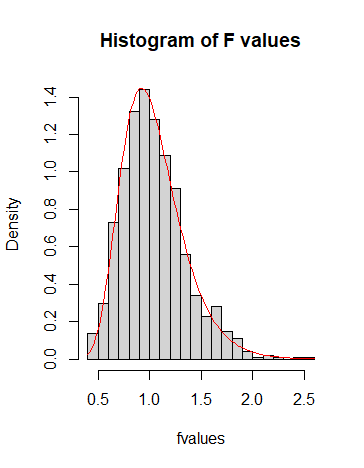
\includegraphics[width=0.55\textwidth]{exercise1a.png}

	\item \begin{lstlisting}
rejections = rep(0, 1000)

for (i in 1:1000) {
	fvalue = getf()
	if (fvalue <= qf(0.005,49,49) | fvalue >= qf(0.995,49,49)) {
	rejections[i] = 1;
	} 
}

sum(rejections)/1000
# > sum(rejections)/1000
# [1] 0.008
	\end{lstlisting}
	We can see that the proportion of rejections is $0.008$, 
	which is approximately $\alpha = 0.01$.
	\item \begin{lstlisting}
getf = function() {
  sampleX = rexp(50, rate=10)
  sampleY = rexp(50, rate=10)
  varX = var(sampleX)
  varY = var(sampleY)
  f = varY/varX
  return(f)
}
...
# > sum(rejections)/1000
# [1] 0.175
	\end{lstlisting}
	\includegraphics*[width=0.4\textwidth]{exercise1c.png}

	The histogram no longer fits the f-distribution and the rejection rate 
	has increased to 0.175.
\end{enumerate}
\newpage 

\subsection*{Exercise 2}
\begin{enumerate}
	\item We have the null hypothesis $H_0: \sigma_X = \sigma_Y$ and
the alternative hypothesis $H_1: \sigma_X \neq \sigma_Y$.
We assume independence and normality of both samples.
\begin{lstlisting}
# Import files
setwd("C:/Users/merri/Documents/MATH-31H/MATH 181B/Homework 2")
regular = unlist(read.csv("regular.csv"))
fast = unlist(read.csv("fast.csv"))

# Calculate F value
varX = var(regular)
varY = var(fast)
#H0 assumes varX = varY, and so f is just varY/varX
f = varY/varX # f = 0.18

# Do rejection check by using quantiles for alpha=0.05
# Two sided since H1 says varX != varY
if (f <= qf(0.025, 9, 9) | f >= qf(0.975, 9, 9)) {
  print("Reject, variances are not equal")
} else {
  print("Fail to reject, variances can be assumed to be equal")
}
# qf(0.025,9,9) = 0.248 and qf(0.975, 9, 9) = 4.03
# Printed "Reject, variances are not equal"
# Therefore we reject the null hypothesis and cannot assume the variances are equal.
	\end{lstlisting}
	We ended up rejecting the null hypothesis since $f = 0.18 < 0.248 = f_{0.025,9,9}$,
	meaning that we cannot assume that the variances are equal.
	\item Since we rejected the null hypothesis,
	we know that a ratio of 1, which is what is assumed by H0, 
	should not be in the CI.
	\item 
	We have that $\mu_X = \mu_Y$ and $H1: \mu_X > \mu_Y$.
	We assume normality from the law of large numbers and 
	independence of the two samples.
\begin{lstlisting}
# Do a HT on H0: mu_X = mu_Y and H1: mu_X > mu_Y.
# We cannot assume that sigma_x = sigma_y,
# so we use Welch's approximation for this calculation.

# Calculate mean and std
Xbar = mean(regular)
Ybar = mean(fast)
Sx = sd(regular)
Sy = sd(fast)
n = length(regular)
m = length(fast)

# The test statistic is 
Tv = (Xbar - Ybar)/sqrt(Sx^2/n + Sy^2/m) # Tv= 0.0726

# v degrees of freedom
v = round((Sx^2/n + Sy^2/m)^2/(Sx^4/n^2/(n-1) + Sy^4/m^2/(m-1)))

# Find P(t_12 > 0.0726)
pt(Tv, v, lower=F)
# Yields value of 0.4716732
	\end{lstlisting}
	Since $p = 0.4716732 > 0.03$, we fail to reject the null hypothesis and 
	we cannot say that the fast glue drys faster that the regular glue.
	\item \begin{lstlisting}
var.test(regular, fast)\$p.value 
# 0.01754406 so reject null hypothesis

var.test(regular, fast)\$conf.int 
# 1.381679 22.395125 so 1 is not in the interval

t.test(regular, fast, alternative = "greater")\$p.value 
# p value of 0.4716667, so fail to reject
	\end{lstlisting}
	\newpage 

	\subsection*{Exercise 3}
	The mean of the confidence interval is -0.08.
	We have that 
	\[
		\frac{23}{50} - \frac{y}{50} = -0.08
	\]
	Therefore $y=27$, meaning Kate cleaned the stove right after cooking 27 times.
\end{enumerate}
\end{document}




